\documentclass[11pt]{standalone}

\usepackage{helvet}

\usepackage{ifthen}
\usepackage{tikz} 
\usetikzlibrary{shapes.misc}
\usetikzlibrary{arrows,arrows.meta}
\usetikzlibrary{calc,intersections, patterns, math}
\usetikzlibrary{decorations.pathmorphing}
\usetikzlibrary{angles,quotes}

\definecolor{pfeil}{RGB}{168,167,167}
\definecolor{petrol}{RGB}{0, 118, 136}
\definecolor{darkgoldenrod}{RGB}{184, 134, 11}
\colorlet{petrol-lighter}{petrol!40}
\colorlet{darkgoldenrod-lighter}{darkgoldenrod!40} 

\begin{document}

\def\scl{0.25}

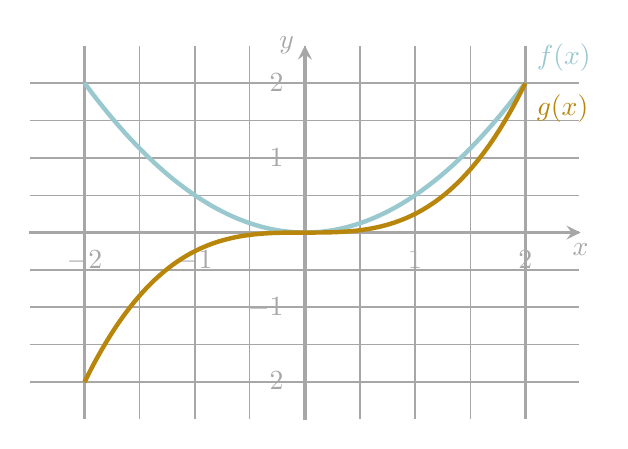
\begin{tikzpicture}[pfeil, yscale=0.95,xscale=1.4,>=stealth]

	% \draw[thick, fill=petrol!20, draw=petrol-lighter, rounded corners=2ex, opacity=0.5] (0,0) rectangle ++ (1.5,3.5);
	% \draw[thick, fill=darkgoldenrod!20, draw=darkgoldenrod-lighter, rounded corners=2ex, opacity=0.5] (5,0) rectangle ++ (1.5,3.5);


	\draw[thin, step=0.5] (-2.49,-2.49) grid (2.49,2.49);
		\draw[thick, step=1] (-2.49,-2.49) grid (2.49,2.49);
		\draw[very thick, -stealth] (-2.5,0) -- (2.5,0) node[below] {$x$}; 
		\draw[very thick, -stealth] (0,-2.5) -- (0,2.5) node[left] {$y$}; 
		\foreach \x in {1,2}{
			\draw[thick] (\x,0) -- ++ (0,-0.1) node[below] {$\x$};
			\draw[thick] (-\x,0) -- ++ (0,-0.1) node[below] {$-\x$};
			\draw[thick] (0,\x) -- ++ (-0.1,0) node[left] {$\x$};
			\draw[thick] (0,-\x) -- ++ (-0.1,0) node[left] {$-\x$};
		}
		\draw[ultra thick, petrol-lighter, domain=-2:2, samples=50, smooth] plot(\x,{1/2*\x*\x}) node[above right] {$f(x)$};
		\draw[ultra thick, darkgoldenrod, domain=-2:2, samples=50, smooth] plot(\x,{1/4*\x*\x*\x}) node[below right] {$g(x)$};


\end{tikzpicture}

\end{document}
